\documentclass[10pt,a4paper,ngerman]{scrartcl}
\usepackage[utf8]{inputenc}
\usepackage[ngerman]{babel}
\usepackage[T1]{fontenc}
\usepackage{amsmath}
\usepackage{amsfonts}
\usepackage{amssymb}
\usepackage{makeidx}
\usepackage{graphicx}
\usepackage{epstopdf}
\usepackage[onehalfspacing]{setspace}
\usepackage{array}
\usepackage{upgreek}
\usepackage{float}
\usepackage{csquotes}
\usepackage{chemformula}
\usepackage{chemgreek}
\usepackage{chemmacros}
\chemsetup{modules=all}
\usepackage{tikz}
\usepackage{siunitx}
\sisetup{locale = DE,per-mode = symbol}
\usepackage{esvect}
\usepackage{geometry}
\usepackage{pdfpages}
\usepackage[font=small]{caption}
%\usepackage[version=4]{mhchem}
\usepackage[backend=biber, style=chem-angew]{biblatex}
\addbibresource{Ionische.bib}
\usepackage{tabularx, booktabs, multirow}
\usepackage[pdfborder={0 0 0}]{hyperref}
\usepackage{scrlayer-scrpage}%Header für die KOMA-script -Klasse
%\usepackage{hyperref}
\usepackage{pgfplots}
\usepackage{textgreek}


\newcommand{\tildenu}{{\fontencoding{LGR}\selectfont\accperispomeni\textnu}}
\captionsetup{format=plain}
\chemsetup[phases]{pos=sub}
\chemsetup[redox]{pos=top}
\chemsetup[redox]{align=center}
%\chemsetup[redox]{explicit-sign=true}
%\chemsetup[redox]{roman=false}
\newcommand{\celsius}{^{\circ}\mathrm{C}}
\parindent0pt
\sloppy
\DeclareChemPhase{\s}{s}
\DeclareChemPhase{\l}{l}
\DeclareChemPhase{\g}{g}
\renewcaptionname{ngerman}{\figurename}{Abb.}
\renewcaptionname{ngerman}{\tablename}{Tab.}
\geometry{bottom=100pt} \geometry{top=80pt}
\newcommand{\m}{\mathrm{m}}
\newcommand{\K}{\mathrm{K}}
\newcommand{\J}{\mathrm{J}}
\newcommand{\gr}{\mathrm{g}}
\newcommand{\kg}{\mathrm{kg}}
\newcommand{\mol}{\mathrm{mol}}
\newcommand{\Pa}{\mathrm{Pa}}
\newcommand{\ad}{\mathrm{ad}}
\newcommand{\de}{\mathrm{de}}
\newcommand{\gmol}{\mathrm{\frac{g}{mol}}}
\newcommand{\JKmol}{\mathrm{\frac{J}{K \cdot mol}}}
\newcommand{\kgmss}{\mathrm{\frac{kg}{m \cdot s^2}}}
\newcommand{\loge}{\mathrm{ln}}


\begin{document}
\begin{titlepage}
	\vspace*{2,5cm}
	\begin{center}
		\begin{LARGE}
			\textbf{Polymer Chemie}\\
			\textbf{Ionische Polymerisation}\\
		\end{LARGE}
		\vspace{1cm}
		\textbf{Universität Stuttgart}\\
		\vspace*{1,5cm}
		\begin{tabular}{lp{7,5cm}l}
			Author 1:     &Laurens Viehoff\\
            Author 2:     &Felix Roth\\   
			E-Mail 1:      &st183688@stud.uni-stuttgart.de\\
            E-Mail 2:      &st188157@stud.uni-stuttgart.de  \\
			Student-ID 1: & 3676761   \\ 
            Student-ID 2: & 3711192 \\ \\
			Assistentin:  &   \\ \\ 
		\end{tabular}
		
		\vspace{2cm}
		Version 2\\
	\end{center}

    
\end{titlepage}
\thispagestyle{empty}
\renewcommand{\thepage}{\arabic{page}}
\newpage
\tableofcontents
\setcounter{page}{1}
\renewcommand{\thepage}{\arabic{page}}
\newpage

 
\section{Theorie}

	Der Kerngedanke der ionischen Polymerisation ist das bilden einer Polymerkette durch Anlagerung der Monomere an 
	ein Makroanion oder Kettenendgruppe. Die Ladung des Makroions entscheidet hierbei darüber ob es sich um eine 
	anionische- oder eine kationische-Polymerisation handelt. Diese Eigenschaften der Endgruppen wird durch das Lösemittel beeinflusst.
	Da die unterschiedliche Dissoziation, die Stabilisierung der Ionenpaare beeinflusst.
	Dadurch wird auch die Verfügbarkeit der effektiven Ladung reguliert.
	Weitere Einflüsse auf die Eigenschaften der Endgruppen hat unteranderem auch der Druck und die Temperatur.
	Der Einfluss des Lösungsmittels ist in Abbildung \ref{Ladungsggw} dargestellt.
	Die Polarität des Lösemittels kann die Ladungen unterschiedlich gut stabilisieren. 
	So stabiliesieren polare Lösemittel solventsgetrennte Ionenpaare, wodurch in polaren Lösemitteln diese bevorzugt vorliegen.

		\begin{figure}[H]
			\centering
			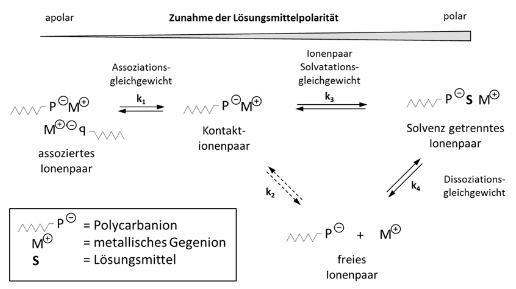
\includegraphics{Bilder/Lösemitteleinfluss.png}
			\caption{Die Abbildung zeigt den Einfluss des Lösemittels auf das Gleichgewicht der Ionen im Falle der anionischen Polymerisation. 
			So Liegen die Ionen im apolare Lösemittel als Ionenpaar vor und im polaren Lösemittel als getrennte Ionenpaare.\cite{polyskript}}
			\label{Ladungsggw}
		\end{figure}

	So ist durch ein vorliegen eines assoziierten Ions die Reaktivität sowie Nukleophilie verringert da die Ladung kompensiert wird
	Die Stärke dieses Ions hat dabei sehr großen Einfluss auf die Wachstumsgeschwindigkeit. 
	So sind gebundene Ionenpaare langsamer in ihrem Wachstum als freie Ionen.\\
	
	Wird die ionische Polymerisation mit z.B. der radikalischen Polymerisation verglichen, wird deutlich,
	dass bei der ionischen Polymerisation die Möglichkeit besteht, diese lebend durchzuführen, da keine bimolekulare Terminierungsreaktionen 
	stattfinden können. 
	Somit kann die Polymerisation theoretisch endlos aufrecht erhalten bleiben, bzw. sie kann durch erneute Zugabe von Monomer weitergeführt werden.
	Diese kann durch eine terminierende Substanz gezielt Terminiert werden, es wird auch von \textquotedblleft Abtöten\textquotedblright \, gesprochen.

	\subsection{Ablauf der lebenden anionischen Polymerisation}

		Die lebende anionische Polymerisation kann wie bei der radikalischen Polymerisation in drei Teile geteilt werden.\\
		Der erste Schritt ist die Initiierung. Hierfür werden bei der anionischen Polymerisation nukleophile oder reduktive Spezies verwendet.
		Hierbei gilt die Regel je weniger elekrophil das Zentrum ist, umso stärker muss die Base sein. Die Elektrophilie wird dabei von der 
		Stabilisierung der konjugierten anionischen Spezies beeinflusst, die negative Ladung wird dabei über -I oder -M-Effekte stabilisiert.
		Beispiele für solche Initiatoren sind Alkalimetalle, Alkylverbindungen der Alkalimetalle und Alkalimetallnaphthalide \cite{polyskript}.
		Im Rahmen dieses Versuchs wurde \textit{sec}-BuLi verwendet. Dabei reagiert dieses nach folgender Reaktionsgleichung:

			\begin{figure}[H]
				\centering
				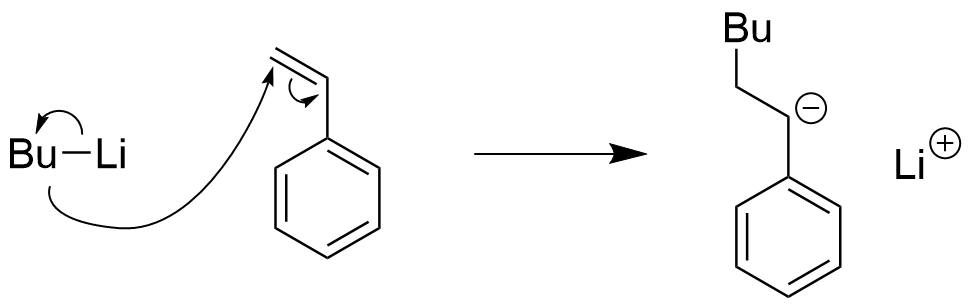
\includegraphics[scale = 0.35]{Bilder/Initiierung.png}
				\caption{Die Abbildung zeigt den Initiatorschritt von Styrol mit \textit{sec}-BuLi.}
				\label{Initiierung}
			\end{figure}

		Eine weitere Methode die Reaktion zu Initiieren ist durch Naphthalin mit einem Alkalimetall. 
		Hierbei wird zuerst ein Radikalanion gebildet, welches anschließend seine Ladung sowie das Radikal an das Monomer (in unserem Fall Styrol) abgibt.
		Das hierraus entstandene radikalanionische Monomer rekombiniert und weist anschließend zwei aktive anionische Enden auf.

			\begin{figure}[H]
				\centering
				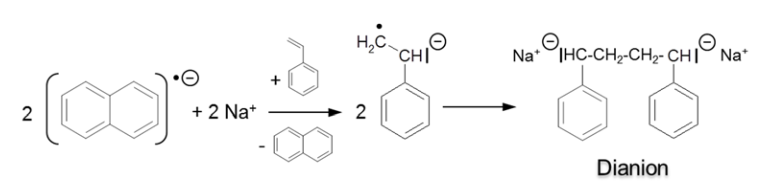
\includegraphics[width = \textwidth]{Bilder/NaphthalinStarter.png}
				\caption{Die Abbildung zeigt die Initiierung von Styrol mit einem Alkalimetallnaphthaliden.\cite{polyskript}}
				\label{NaphthalinStarter}
			\end{figure}
		
		
		Nach der Initiierung findet das Kettenwachstum statt, auch gezeigt in Abbildung \ref{Wachstum}.

			\begin{figure}[H]
				\centering
				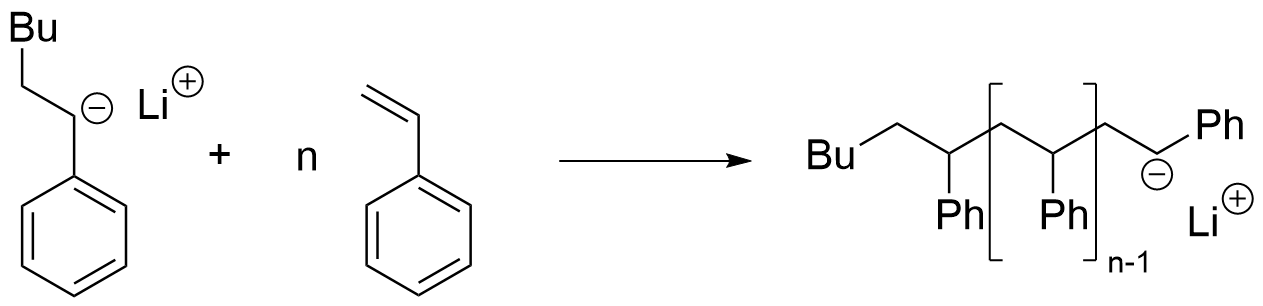
\includegraphics[scale = 0.3]{Bilder/Wachstum.png}
				\caption{Die Abbildung zeigt den Allgemeinen Wachstumsschritt anhand des Beispiels von Styrol.}
				\label{Wachstum}
			\end{figure}


		Dieses Wachstum hat am meisten Einfluss auf die Reaktionskinetik der Polymerisation. 
		So ergibt sich der gemittelte Polymerisationsgrad $\bar{P}_\text{n}$ wie folgt:

			\begin{equation}
				\bar{P}_\text{n} = \frac{[M]_0 - [M]_t}{[I]}
				\label{Polymerisationsgrad}
			\end{equation}

		Hierbei ist $[M]_0$ die Monomerkonzentration zu Beginn (t=0), $[M]_\text{t}$ ist die Monomerkonzentration zu dem Zeitpunkt t
		und $[I]$ ist die Initiatorkonzentration. Aus $\bar{P}_\text{n}$ lässt sich der Polydispersitätsindex (\DH) berechnen. 
		Er beschreibt die Breite der Poisson-Verteilung der Molmassenverteilung und ist durch folgende Gleichung gegeben:

			\begin{equation}
				\text{\DH} = \frac{\bar{P}_w}{\bar{P}_n} = \frac{\bar{M}_w}{\bar{M}_n} = 1 + \frac{1}{\bar{P}_n}
			\end{equation}
			
\newpage
		Hierbei ist $\bar{M}_w$ das gewichtsmittlere Molekulargewicht, $\bar{M}_n$ das zahlenmittlere Molekulargewicht,
		$\bar{P}_n$ der zahlenmittlere Polymerisationsgrad und $\bar{P}_w$ der gewichtsmittlere Polymerisationsgrad. 
		Dabei gilt, welches das synthetische Polymer mit einem Polymerisationsgrad gegen unendlich den PDI von 1 zu haben.
		Dabei ist wichtig, dass dies lediglich ein theoretischer Wert ist und nicht realisierbar ist.
		Realisierbar sind dabei nur Werte größer als 1.\\\\

		Zuletzt findet der gezielte Abbruch der Polymerisation statt. 
		Dabei wird nur von nicht lebender Polymerisation gesprochen da die lebendende Polymerisation keinen Abbruch besitzt.
		Die Carbanionen werden in der Regel mit schwächeren Säuren wie Methanol oder Wasser abgebrochen.
		Hierbei findet eine Veränderung der chemischen Eigenschaften des Polymers statt, 
		da durch Verwendung von unterschiedlichen Abbruchreagenzien die Endgruppe gewählt wird.
		So führt Beispielsweise ein Abbruch mit \ch{CO2} zu einer Carboxylgruppe als Endgruppe [\ref{Abbruch}].

			\begin{figure}[H]
				\centering
				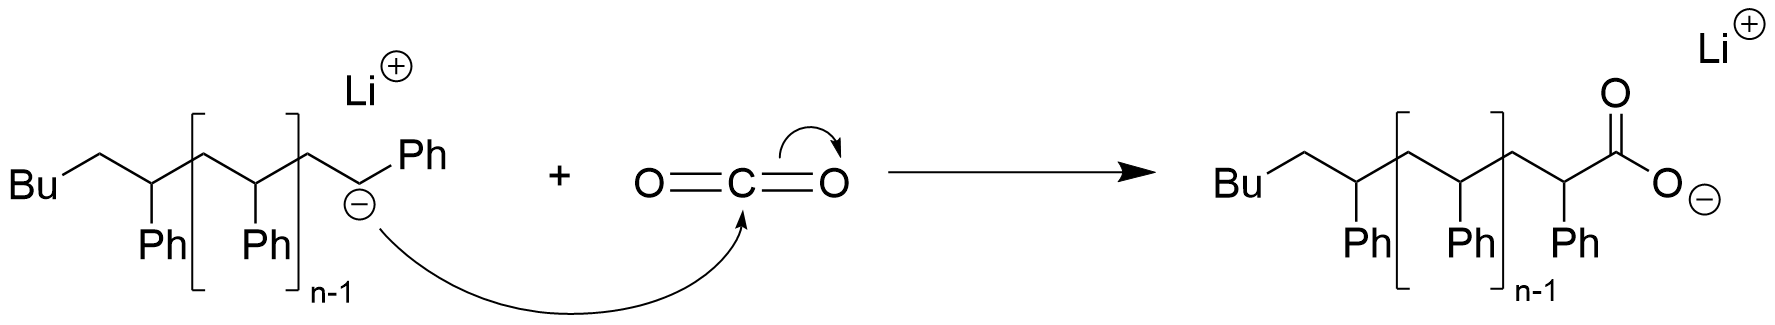
\includegraphics[width = \textwidth]{Bilder/Abbruch.png}
				\caption{Die Abbildung zeigt den Mechanistischen Abbruch der Polymerisation mittels \ch{CO2}.}
				\label{Abbruch}
			\end{figure}

			

\section{Durchführung}

	Innerhalb des gesamten Versuchs wurde unter Schlenk Bedingungen gearbeitet.\\
	In einem Schlenkzweihals mit glasummanteltem Rührfisch wurde Toluol (\SI{40,0}{ml}) und Styrol (\SI{3,00}{ml}, \SI{26,2}{mmol}, 1,00 Äq) vorgelegt und 
	auf \SI{50}{\degreeCelsius} hochgeheizt.
	Anschließend wurde \textit{sec}-Butyllithium in Cyclohexan (\SI{0,30}{ml}, \SI{1,40}{\frac{mol}{l}}, \SI{0,42}{mmol}, 0,02 Äq) zugegeben.
	Nach 30 min wurde Isopren (\SI{2,00}{ml}, \SI{20,0}{mmol}, 0,76 Äq) zugegeben und weitere 2 h gerührt. 
	Zur terminierung der Reaktion wurde Methanol (\SI{0,50}{ml}) zu der Lösung gegeben, 
	in ca. \SI{400}{ml} Methanol gefällt und im Vakuumtrockenschrank getrocknet.


\newpage

\section{Auswertung}
 
	Bei der Synthese wurden $\SI{2,61}{g}$ des Copolymers erhalten. Dieses wurde aus \SI{2,73}{g} Styrol und \SI{1,36}{g} Isopren synthetisiert, womit sich eine Ausbeute von 
	\begin{equation*}
		\sigma = \frac{m_\text{Copo}}{m_\text{Styrol} + m_\text{Isopren}} = \frac{\SI{2,61}{g}}{\SI{2,73}{g} + \SI{1,36}{g}} = 0,639 = 63,9\%
	\end{equation*}
	ermittelt. \\
	Nach Ermittlung der Massen durch GPC konnte folgende Kurve erhalten werden:

		\begin{figure}[H]
			\centering
			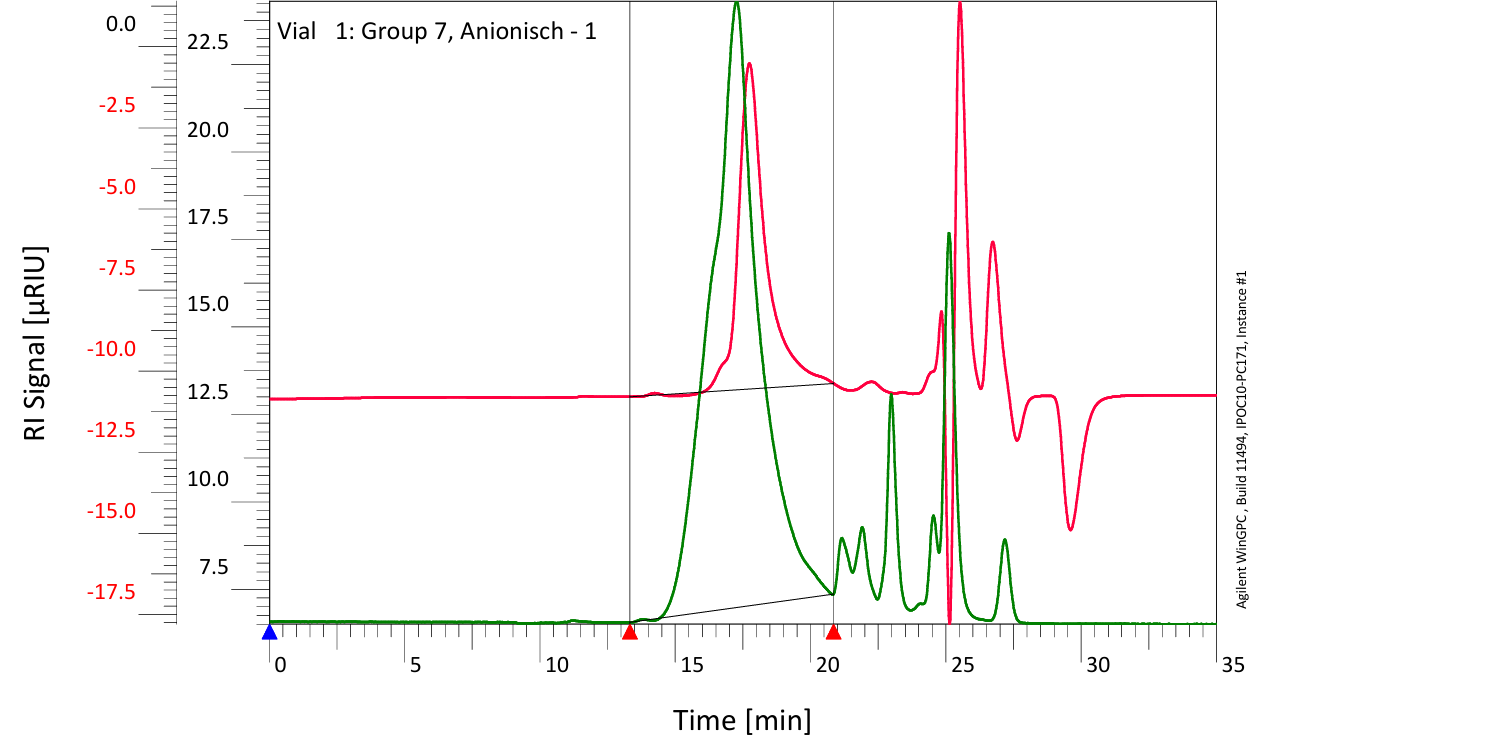
\includegraphics[scale = 0.4]{Bilder/AnionischeKurve.png}
			\caption{Die Abbildung zeigt die GPC-chromatografie zu dem erhaltenen Copolymer.}
			\label{GPCKurve}
		\end{figure}

	Bei dem Chromatogramm sind einige Signale zu erkennen, die auf unterschiedliche Polymerkettenlängen, aber auch auf Monomer oder Lösungsmittel
	zurückzuführen sind. Das erste Signal bei zwischen 15 und 20 min ist dabei den Polymeren zuzuorden und die Signale, die später auftreten, sind 
	durch Monomer oder Lösungsmittel verursacht. Die verschiedenen Kurven sind dabei durch zwei Detektoren aufgenommen, wovon die grüne Kurve 
	durch einen UV/Vis Detektor aufgenommen wurde und die blaue Kurve durch einen RI-Detektor aufgenommen wurde. Der RI Detektor misst dabei 
	die Änderung des Brechungsindex der Lösung und bestimmt darüber das Molekulargewicht und die Konzentration der Polymerketten.\\

	So konnte über den RI-Detektor eine zahlenmittlere Molmasse von M$_\text{n} = \SI{21660}{g/mol}$ und eine gewichtsmittlere Molmasse von 
	M$_\text{w} = \SI{27060}{g/mol}$ bestimmt werden. Die ermittelten Molekulargewichte führen zu einem Polydispersitätsindex von \DH = 1,25. 
	Der Polydispersitätsindex von 1,25 ist dabei ein erwartbarer Wert, da es sich bei der anionischen Polymerisation um eine lebende Polymerisation 
	handelt und dabei das Molekulargewicht kontrollierbar ist. Allerdings bedeuten Werte größer als 1, dass es sich um eine Verteilung von 
	Molekulargewichten handelt. Diese Verteilung kann auch in der GPC Kurve erkannt werden, da die Kurve zwischen 15 und 20 min nicht unendlich 
	scharf ist, sondern eine gewisse Breite aufweist. Die Werte von M$_\text{n}$ und M$_\text{w}$ sind dabei verschieden voneinander, da diese 
	anders berechnet werden. Bei der gewichtsmittleren Molmasse gehen die schweren Molmassen mehr in das Gewicht ein, da es quadratisch gewichtet wird. 
	Bei der zahlenmittleren Molmasse werden alle Moleküle gleich gewichtet, wodurch ein kleineres Molekulargewicht herauskommt.

	
	Das zahlenmittlere Molekulargewicht kann auch theoretisch berechnet werden.
	Dabei wird wie folgt vorgegangen:

		\begin{equation}
			\bar{M_n} = \frac{\sum m_\text{Monomer}}{n_\text{Initiator}} = \frac{\SI{2,7}{g} + \SI{1.36}{g}}{\SI{0.42}{mmol}} = \SI{9666,67}{\frac{g}{mol}} 
		\end{equation}

	Die theoretische Molmasse ist um einiges geringer als die experimentell ermittelte Molmasse. 
	Das liegt daran, dass die theoretische Molmasse von einem kompletten Umsatz des Initiators ausgeht. Dieser kann aber durch Wasser- oder 
	Sauerstoffverunreinigungen verringert werden, wodurch die Stoffmenge an Initiator abnimmt und somit die Molmasse steigt. Dadurch, dass 
	die theoretische Molmasse um etwa die Hälfte niedriger ist, entspricht das einem Initiatorumsatz von ebenfalls etwa 50 \%.
	Desweiteren kann es auch daran liegen, dass eine Kettenverdopplung durch Sauerstoff im System stattgefunden hat.


\section{Fragen}

	\subsection{Frage 1}

		Die zahlenmittlere Molmasse lässt sich durch folgende Gleichung beschreiben:

		\begin{equation}
			\bar{M_n} = \frac{\sum m_\text{Monomer}}{n_\text{Initiator}}
		\end{equation}

	\subsection{Frage 2}

		Die Stoffmenge an Methanol zum abbrechen, entspricht derselben des Initiators. Über die molekulare Masse und Dichte von Methanol wird 
		das benötigte Volumen zu $\SI{17,034}{\mu l}$ berechnet. 

	\subsection{Frage 3}

		Da Toluol am ahnlichsten zu Styrol ist und sich Styrol darin gut löst. 
		Im Vergleich zu Benzol ist es ungefährlicher im Umgang.
		Bei THF ist das Problem in der Polarität da THF sehr Polar ist und Toluol unpolar. Daher wird das Toluol lieber verwendet da dieses polarer und Aromatisch ist.
		Bei Heptan liegt ein Löslichkeitsproblem vor, da es sich hierei um ein lineares Alkan handelt und es sich bei Styrol um einen Aromaten handelt.
		Dabei gilt \dq Gleiches in Gleichen\dq.


	\subsection{Frage 4}

		Die Reaktionen sind in den Abbildungen [\ref{Initiierung} - \ref{Abbruch}] zu sehen.

	\subsection{Frage 5}

		Die einzige denkbare Nebenreaktion wäre ein Abbruch durch Verschmutzung wie zB. \ch{CO2}, \ch{H2O} oder \ch{O2}.

	\subsection{Frage 6}

		Bei der ionischen Polymerisation besteht die Möglichkeit, dass die ionischen Enden (lebnenden Enden) nicht als freie Ionen vorliegen sondern
		als Aggregate. Dabei gilt, je mehr Aggregate gebildet werden desto langsamer ist das Wachstum der Polymerisation.

	\subsection{Frage 7}

		\begin{figure}[H]
			\centering
			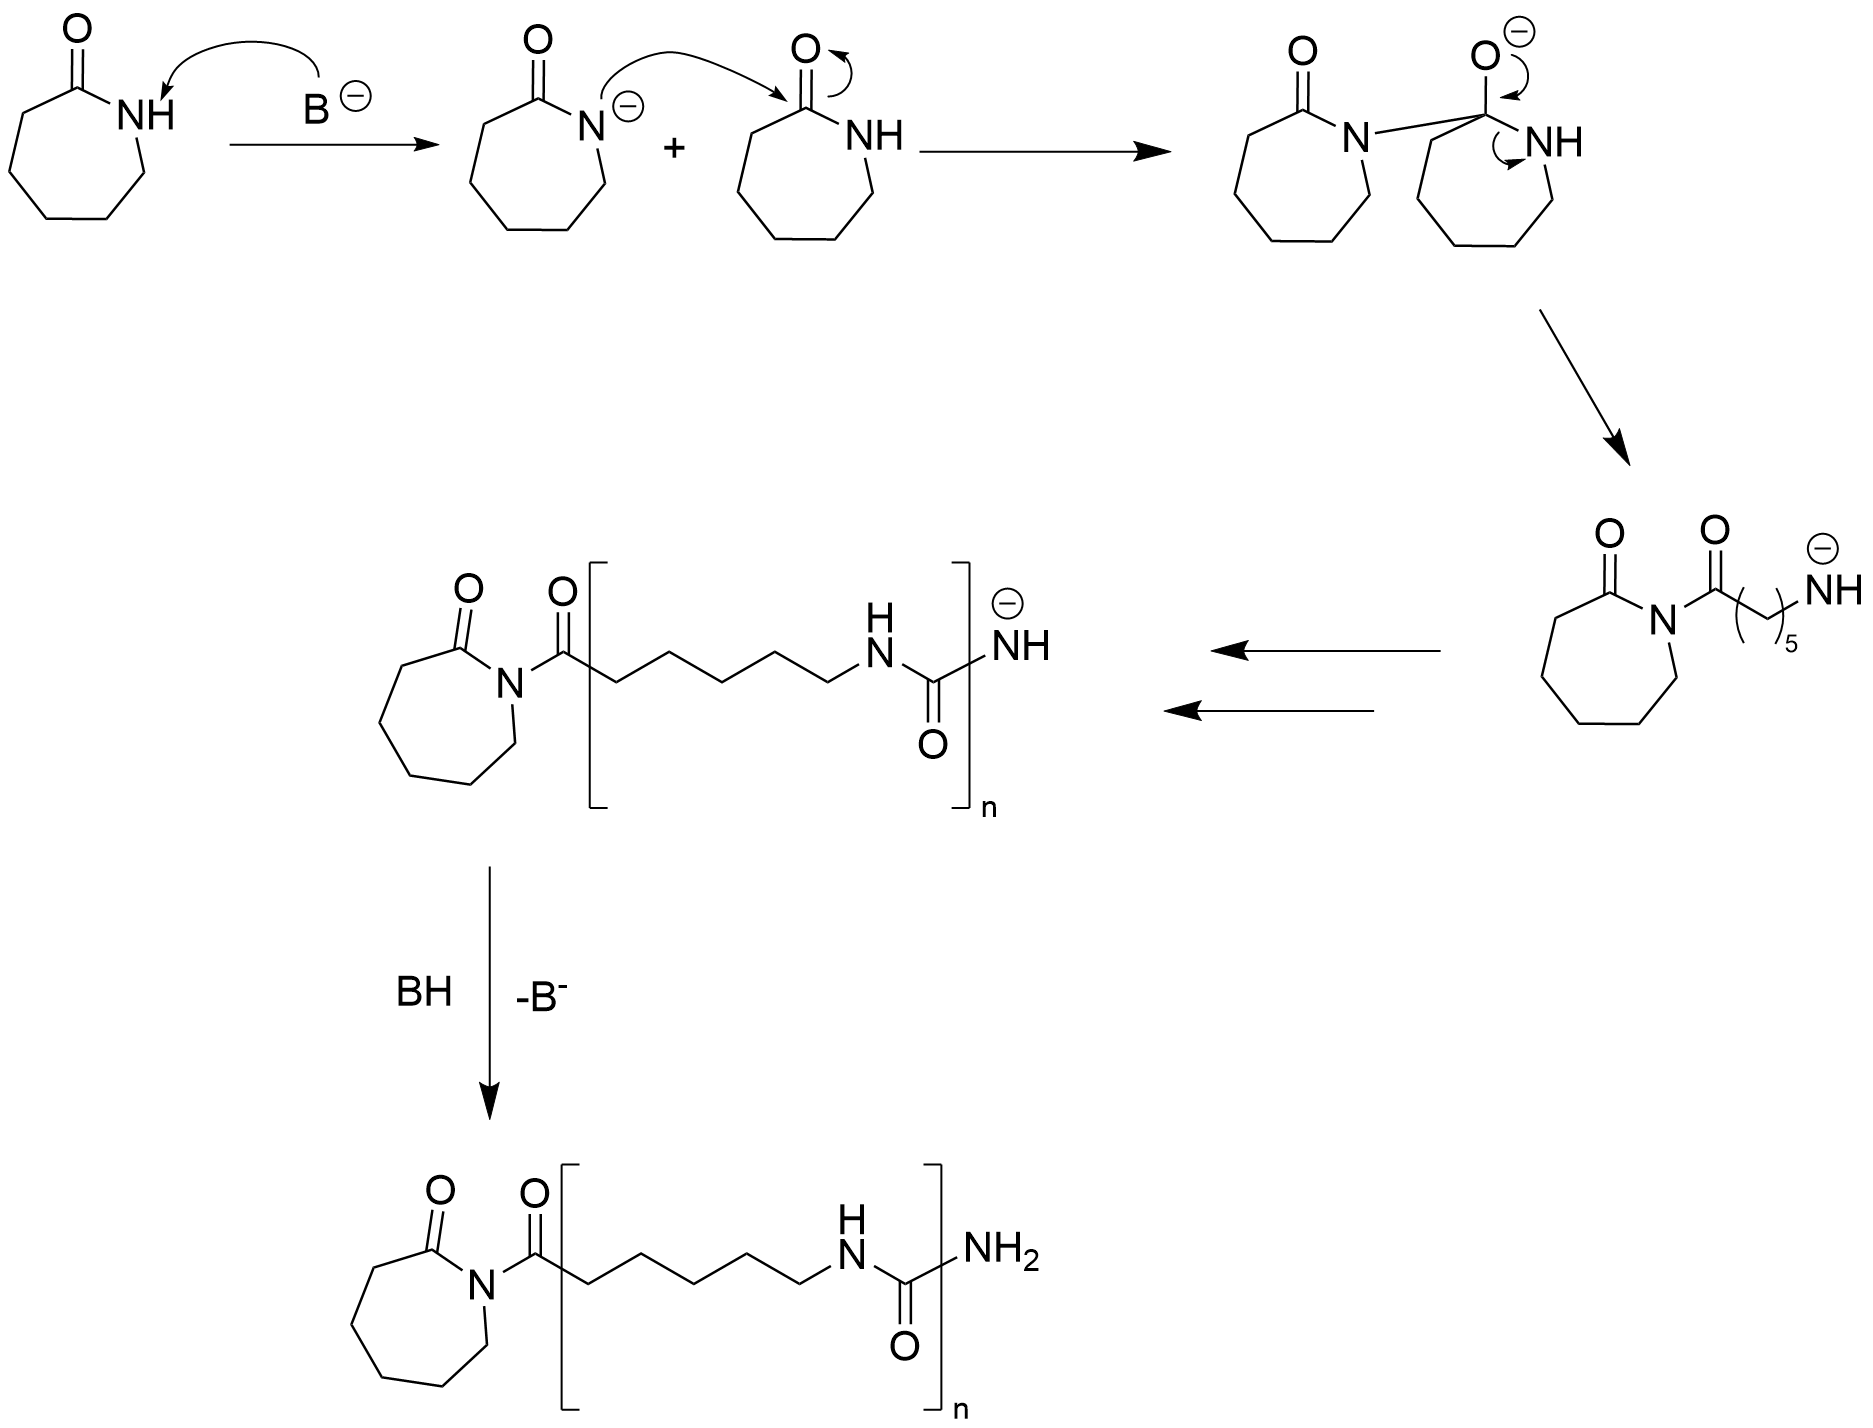
\includegraphics[scale = 0.25]{Bilder/Nylon6.png}
			\caption{Die Abbildung zeigt die ringöffnende Polymerisation von $\epsilon$-Caprolactam zu Nylon-6.}
			\label{Nylon6}
		\end{figure}

	\subsection{Frage 8}

		Die Synthese von SBS erfolgt über die anionische Polymerisation, mit Initiietung über Naphthylnatrium von Butadien. Dadurch bildet sich das 
		in Abbildung \ref{NaphthalinStarter} zu sehende Dianion und endgültig eine dianionische Polymerkette. Anschließend wird 
		die gewünschte Menge an Styrol zugegeben, um das Blockcopolymer SBS zu synthetisieren. 


\printbibliography

\end{document}

